\documentclass[11pt, A4paper, norsk]{article}
\usepackage{amsfonts}
\usepackage{amsmath}
\usepackage{amssymb}
\usepackage{amsthm}
\usepackage{babel}
\usepackage{cite}
\usepackage{color}
\usepackage{float}
\usepackage[T1]{fontenc}
\usepackage{graphicx}
\usepackage[colorlinks]{hyperref}
\usepackage[utf8]{inputenc}
\usepackage{listings}
\usepackage{textcomp}


\definecolor{dkgreen}{rgb}{0, 0.6, 0}
\definecolor{gray}{rgb}{0.5, 0.5, 0.5}
\definecolor{daynineyellow}{rgb}{1.0, 0.655, 0.102}
\definecolor{url}{rgb}{0.1, 0.1, 0.4}

\lstset{frame=tb,
	language=Python,
	aboveskip=3mm,
	belowskip=3mm,
	showstringspaces=false,
	columns=flexible,
	basicstyle={\small\ttfamily},
	numbers=none,
	numberstyle=\tiny\color{gray},
	keywordstyle=\color{blue},
	commentstyle=\color{daynineyellow},
	stringstyle=\color{dkgreen},
	breaklines=true,
	breakatwhitespace=true,
	tabsize=3
}

\lstset{inputpath="C:/Users/Torstein/Documents/USN/IIA3120"}
\graphicspath{{C:/Users/Torstein/Documents/USN/IIA3120/}}
\hypersetup{colorlinks, urlcolor=url}

\author{Torstein Solheim Ølberg}
\title{Lab Report for Exercise 1 in IIA3120}



%\lstinputlisting{Filnavn! type kodefil}
%\includegraphics[width=12.6cm, height=8cm]{Filnavn! type png}



\begin{document}
	\maketitle

I have set up a virtual simulation of a UR10 \cite{UR10} 6 axis robot using MatLab with Simulink and Simscape and the urdf and geomitry files found at \cite{URDF}. The simulation can be seen in figure \ref{fig:sim} where the controlling sliders for each joint is on the left, and the image of the robot is after each joint has been changed a little away from zero.
	\begin{figure}[h!]
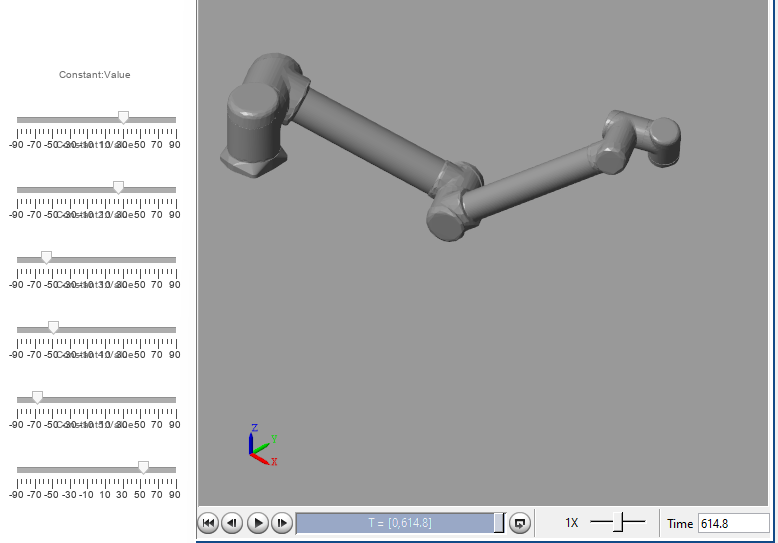
\includegraphics[width=13cm, height=8cm]{Robot_Sliders.png}
\caption{Simulation of the UR10 robot arm after it was moved a little in each joint. The sliders on the left control the joints, starting from one at the top, to six at the bottom.}
\label{fig:sim}
	\end{figure}
To test the model I have chosen to make it move in a trajectory starting at (-0.5, -0.5, -0.5), moving through the point (0.15, 0.7, 0.34) and ending at (0.5, 0.7, 0.5), moving in a polynomial line generated by the MatLab function cubicpolytraj. The resulting trajectory can seen alongside a rendering of the robot, and the two points the robot must pass through, can be seen in figure \ref{fig:traj}.
	\begin{figure}[h!]
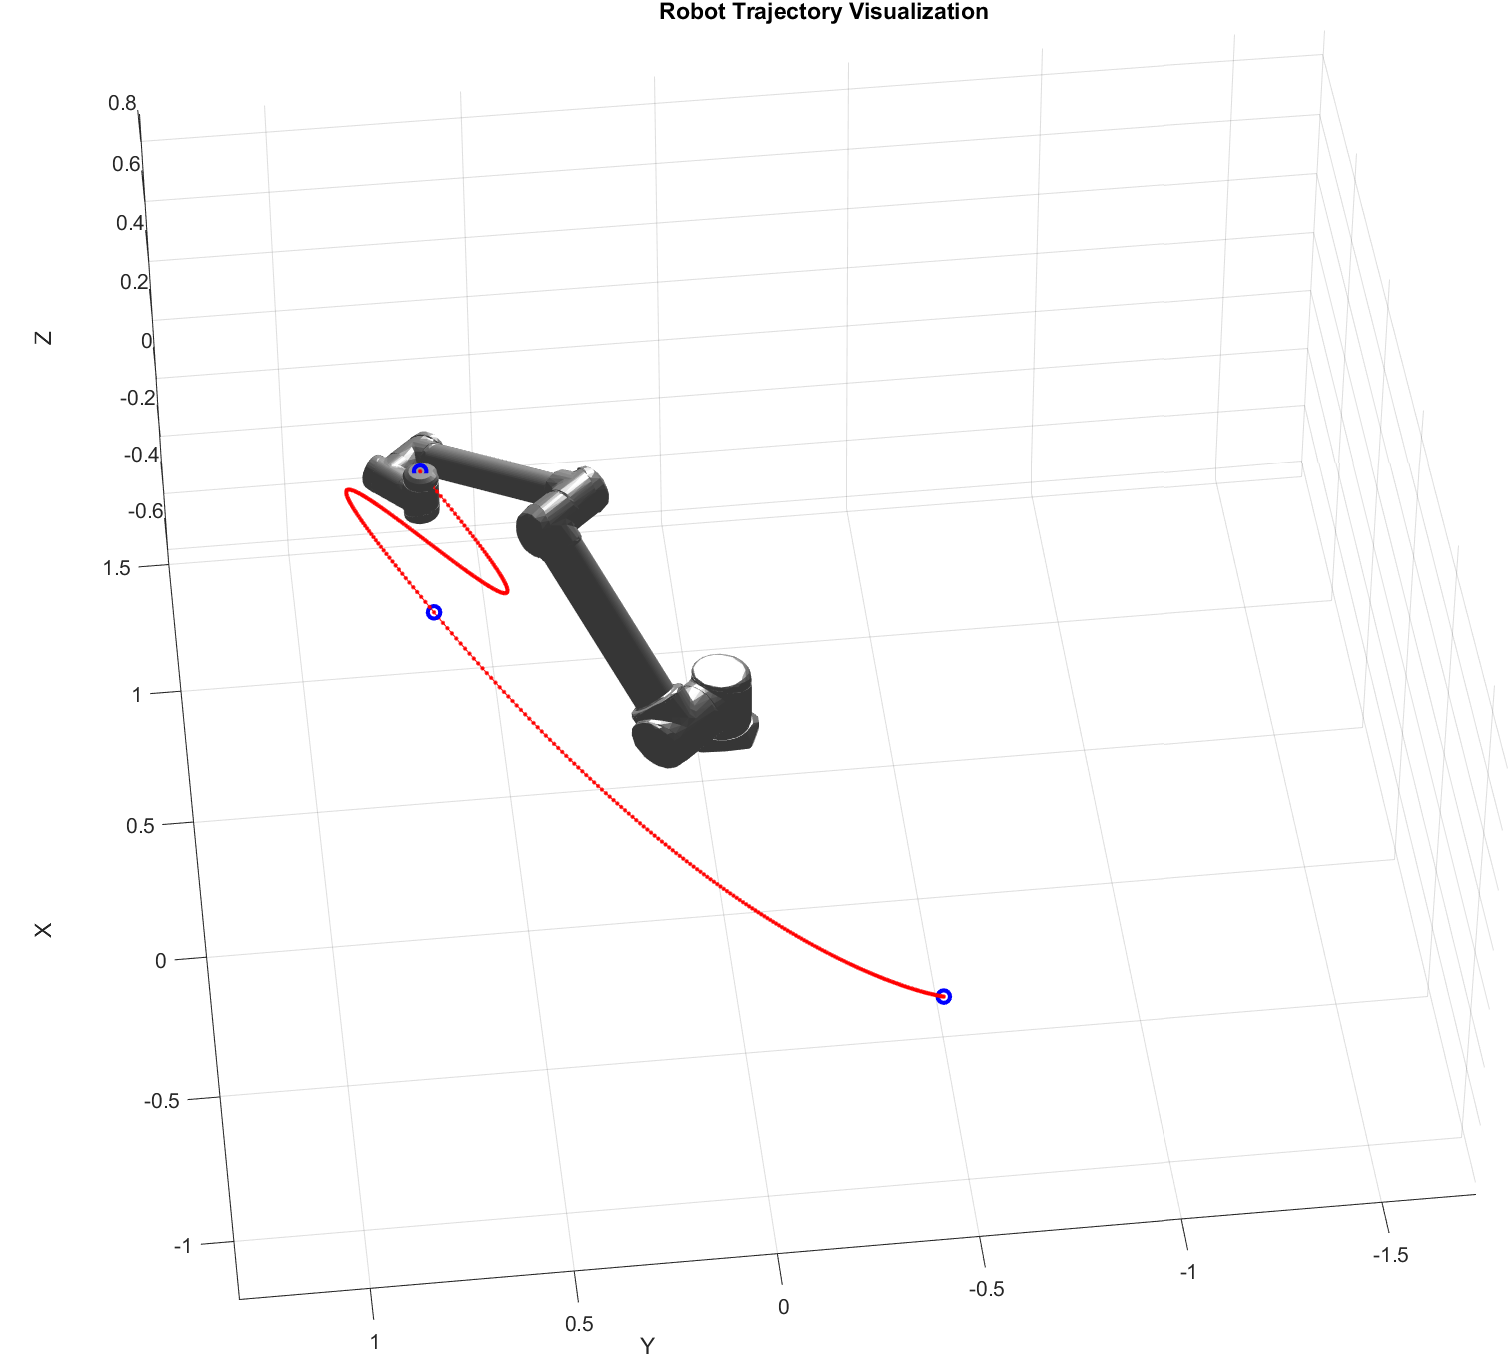
\includegraphics[width=13cm, height=8cm]{Trajectory figure.png}
\caption{Rendering of the UR10 robot with a trajectory to follow marked as a red line and two points the robot must move through as blue circles. The circle furthest to the right is the starting point.}
\label{fig:traj}
	\end{figure}
The right most point in the plot is the start point. Along with this rapport, a video of the robot following the path has been submitted.

	\addcontentsline{toc}{chapter}{Bibliography}
	\begin{thebibliography}{9}
		\bibitem{UR10}
Universal Robots. "UR10e" (2024), [Online]. Avaliable: \url{https://www.universal-robots.com/products/ur10-robot/}. (accessed: 12.09.2024) \\
		\bibitem{URDF}
K. Hawkins. [Online]. Avaliable: \url{https://web01.usn.no/~roshans/cfr/downloads/UR10-urdf-geometry.zip}. (accessed: 12.09.2024)
	\end{thebibliography}
\end{document}